\documentclass[12pt, a4paper]{report}

% Essential packages
\usepackage[utf8]{inputenc}
\usepackage[T1]{fontenc}
\usepackage{graphicx}
\usepackage{hyperref}
\usepackage[margin=2.5cm]{geometry}
\usepackage{listings}
\usepackage{xcolor}
\usepackage{float}
\usepackage{amsmath}
\usepackage{caption}
\usepackage{subcaption}
\usepackage{listings}
\usepackage{xcolor}

\lstdefinelanguage{HCL}{
  morekeywords={module,resource,variable,output,provider,terraform},
  sensitive=false,
  morecomment=[l]{//},
  morecomment=[s]{/*}{*/},
  morestring=[b]",
}

\lstset{
  language=HCL,
  basicstyle=\ttfamily\footnotesize,
  keywordstyle=\color{blue}\bfseries,
  stringstyle=\color{red},
  commentstyle=\color{gray}\itshape,
  breaklines=true,
  captionpos=b
}

% Code listing settings
\definecolor{codegreen}{rgb}{0,0.6,0}
\definecolor{codegray}{rgb}{0.5,0.5,0.5}
\definecolor{codepurple}{rgb}{0.58,0,0.82}
\definecolor{backcolour}{rgb}{0.95,0.95,0.92}

\lstdefinestyle{mystyle}{
    backgroundcolor=\color{backcolour},   
    commentstyle=\color{codegreen},
    keywordstyle=\color{magenta},
    numberstyle=\tiny\color{codegray},
    stringstyle=\color{codepurple},
    basicstyle=\ttfamily\footnotesize,
    breakatwhitespace=false,         
    breaklines=true,                 
    captionpos=b,                    
    keepspaces=true,                 
    numbers=left,                    
    numbersep=5pt,                  
    showspaces=false,                
    showstringspaces=false,
    showtabs=false,                  
    tabsize=2
}
\lstset{style=mystyle}

% Introduction% Introduction
%   Background - Abstract
%   the project idea
%   Our goal - objectives
% Literature Review
%   Already existing solutions
%   Missing solutions - gap
%   What will we do - visual programming tool that combines both approaches
% Methodology
%   Overview of the system
%   every drawing we have
%   Backend Architecutre:
%       Why we used ddd, microservices, kubernetes, terraform, asp.net, python service, databases, deployment
%   Frontend Architecutre: ...
% Testing and Evaluation
%   what api endpoints have we implemented in the backend
%   testing these endpoints and adding all the validation
%   talk about the code, some of the important snippets
% Results and Discussion
%   Frontend interfaces
%   discussion of the result
%   did it work ?
%   how quick it is
%   how expensive it is
%   future work ?
% Conclusion and Recommendations
%   short conclusion
%   sahej
% References
%   websites, papers
% Appendices
%   github repositories



% Document Info
\title{
    
\includegraphics[height=5cm]{assets/NNU_Logo.png} \\[1cm]
    
\includegraphics[height=2.5cm]{assets/FlowX_Logo.png} \\[1cm]
    FlowX: A Visual Building Tool that Merges Static Chatbot Flows with Dynamic LLM Responses
}
\author{
    Izzat Alsharif \\
    Amjad Kayed
    \\\\
    \textbf{Supervisor:} Dr. Amjad Abu Hassan
}
\date{January 31, 2025}

\begin{document}

% Front matter
\maketitle
\tableofcontents
\listoffigures
\listoftables

% Abstract
\begin{abstract}
This thesis presents FlowX, ...
\end{abstract}


\chapter{Introduction}

\section{Background}
Chatbots have become a cornerstone of modern digital interactions, bridging the gap between businesses and users through automated, yet personalized communication. Initially designed as rule-based systems with rigid decision trees, chatbots have evolved into dynamic agents powered by artificial intelligence (AI) and natural language processing (NLP). Despite this evolution, the current landscape of chatbot development tools remains fragmented. Solutions today are polarized: they either focus on static, flow-based designs (e.g. ManyChat, Chatfuel) or fully AI-driven interactions (e.g., Dialogflow, Rasa), with few attempts to integrate both approaches effectively. This divide limits developers' ability to create chatbots that are both predictable in structured workflows and adaptable to dynamic user input. Furthermore, existing tools often lack critical features such as advanced customization, extensibility through marketplaces, and flexible deployment options—gaps that hinder innovation and scalability in chatbot development.

\section{Terminology}
To ensure clarity throughout this report, key terms and concepts are defined below:

\subsection{Core Concepts}
\begin{itemize}
    \item \textbf{Chatbot}: A software application designed to simulate human conversation through text or voice interactions, often used for customer support, information retrieval, or task automation.
    
    \item \textbf{Static Workflow}: A predefined conversation path using decision trees and fixed responses, offering predictable and structured interactions.
    
    \item \textbf{Dynamic Routing}: The ability to determine conversation flow based on AI analysis of user intent rather than predefined rules.
    
    \item \textbf{Hybrid Approach}: The combination of static workflows with dynamic, AI-powered interactions in a single chatbot system.

\end{itemize}

\subsection{Technology Stack}
\begin{itemize}
    \item \textbf{LLM (Large Language Model)}: Advanced AI models trained on vast datasets to generate human-like text and understand context.
    
    \item \textbf{LangChain}: A framework for developing applications powered by language models, used in our executor service.
    
    \item \textbf{Microservices}: An architectural style where the application is structured as a collection of loosely coupled services.
    
    \item \textbf{gRPC}: A high-performance RPC (Remote Procedure Call) framework used for communication between services.
    
    \item \textbf{Infrastructure as Code (IaC)}: The practice of managing and provisioning infrastructure through code rather than manual processes.
\end{itemize}

\subsection{Development Concepts}
\begin{itemize}
    \item \textbf{No-Code/Low-Code}: Development approach that enables users to create applications through visual interfaces rather than traditional programming.
    
    \item \textbf{Visual Builder}: A drag-and-drop interface for creating and modifying chatbot workflows without coding.
    
    \item \textbf{Visual Editor}: Interface for customizing the chatbot's appearance and user interface elements.
\end{itemize}

\section{Objectives}
The primary objectives of this work are:
\begin{itemize}
    \item \textbf{To analyze existing chatbot development tools} and identify gaps in their ability to combine static workflows with dynamic adaptability, customization, extensibility and deployment options.
    
    \item \textbf{To design and develop FlowX}, a visual building tool that integrates static, rule-based workflows with dynamic, LLM-powered interactions, addressing the identified gaps.
    
    \item \textbf{To provide advanced customization tools} for chatbot design, allowing users to customize layouts, colors, fonts, and interactive elements to align with brand identity and user experience goals.
    
    \item \textbf{To create a marketplace ecosystem} for sharing, discovering and extending chatbot functionalities, fostering collaboration and reuse.
    
    \item \textbf{To simplify deployment} through flexible publishing options, including API integration and marketplace listings, ensuring accessibility across platforms.
\end{itemize}

\section{Summary}
FlowX addresses critical gaps in the chatbot development landscape by offering a unified platform that combines structured workflows with dynamic adaptability. Its emphasis on customization, extensibility, and ease of use makes it accessible to both technical and non-technical users, democratizing the creation of intelligent chatbots. By bridging the divide between static and AI-driven approaches, FlowX has the potential to improve scalability, reduce development costs, and improve user engagement across industries such as e-commerce, healthcare, and customer service.


\chapter{Literature Review}
\label{chap:literature_review}

\section{Introduction}
Chatbot building tools have evolved from simple rule-based systems to AI-driven dynamic agents. However, most existing solutions focus either on static flow-based designs or fully AI-driven interactions, lacking a seamless integration of both approaches. This chapter reviews existing chatbot builders, automation platforms, and AI-driven chatbot frameworks to identify the gaps that FlowX aims to address.

\section{Theoretical Foundations}

\subsection{Rule-based Chatbots}

Rule-based chatbots follow predefined decision trees or workflows to respond to user input. These chatbots are deterministic and rely on explicit rules to generate responses. For example, a rule-based chatbot might ask a series of questions to gather information from the user and provide a specific response based on the answers. The next figure~\cite{medium_image} shows an example of a rule-based chatbot conversation flow diagram. It consists of a series of nodes representing decision points and transitions between them based on user input.
\begin{figure}[ht]
    \centering
    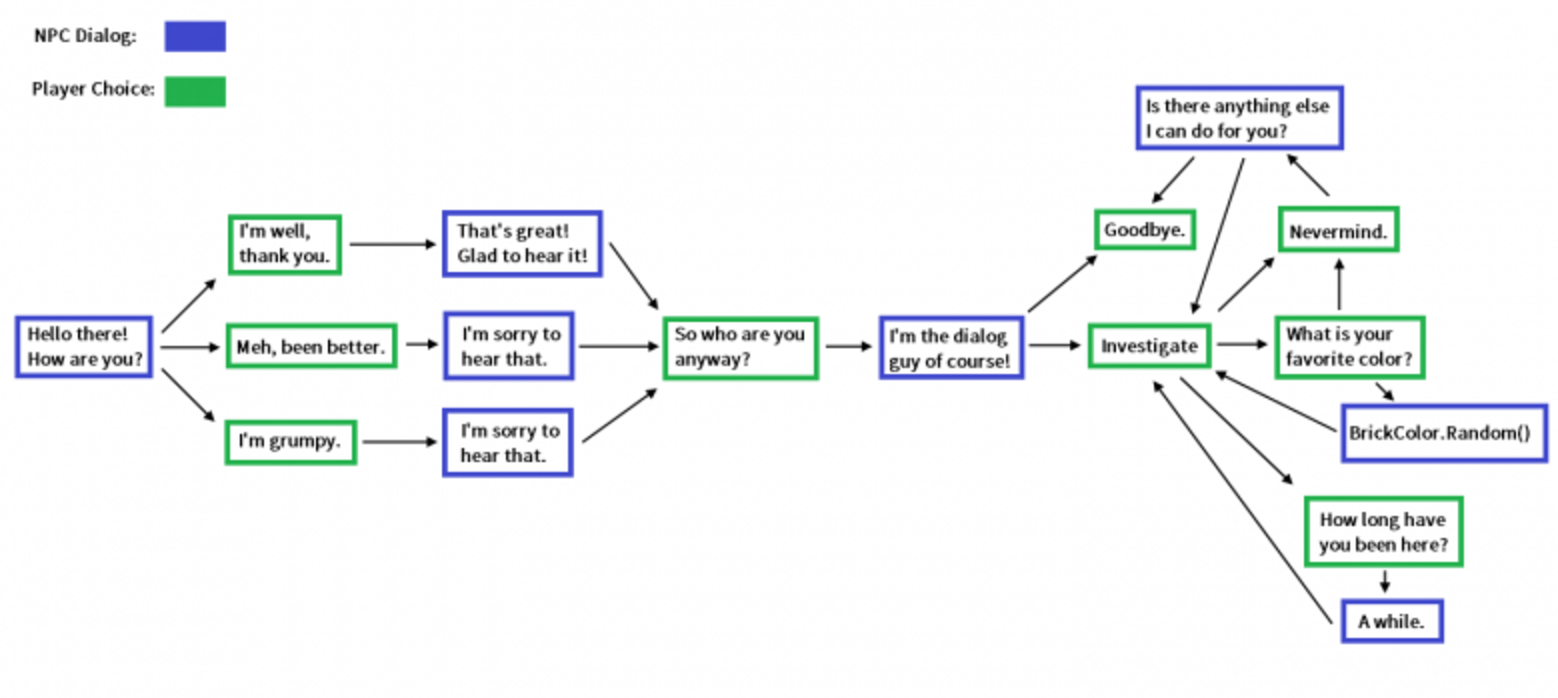
\includegraphics[width=0.7\textwidth]{assets/ChatbotConversationFlowExample.png}
    \caption{Example of a chatbot conversation flow diagram}
    \label{fig:chatbot_flow}
\end{figure}

\subsection{Generative Chatbots}

Generative chatbots leverage large language models (LLMs) like GPT-4 or Claude 3.5 Sonnet to produce contextually relevant responses. Unlike rule-based systems, these chatbots are probabilistic and generate outputs by learning patterns from training data, enabling flexible, open-ended interactions.

The next figure shows an example of a generative chatbot response generated by an LLM. In this example, the user input "explain how a combustion engine works" prompts the chatbot to generate a relevant response based on the context of the conversation.

\begin{figure}[ht]
    \centering
    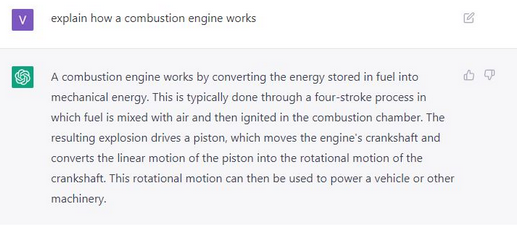
\includegraphics[width=0.7\textwidth]{assets/ChatgptMessageExample.png}
    \caption{Screenshot of a message from ChatGPT.}
    \label{fig:chatgpt_message}
\end{figure}

\subsection{Dynamic Routing}

Dynamic routing refers to the process where a system, such as a chatbot powered by a large language model (LLM), dynamically selects one of several predefined options or pathways based on the context of the user input. Instead of following a rigid, rule-based decision tree, the LLM evaluates the input and chooses the most appropriate response or action from a set of predefined choices. This allows for more flexible and context-aware interactions while still maintaining some level of control over the chatbot's behavior.

The next figure shows an example of dynamic routing in a chatbot conversation. The user gives a textual input, and the LLM evaluates it to determine what option to choose out of two possible responses. This gives the flow structure and more control over the conversation while still allowing for dynamic user interactions.

\begin{figure}[ht]
    \centering
    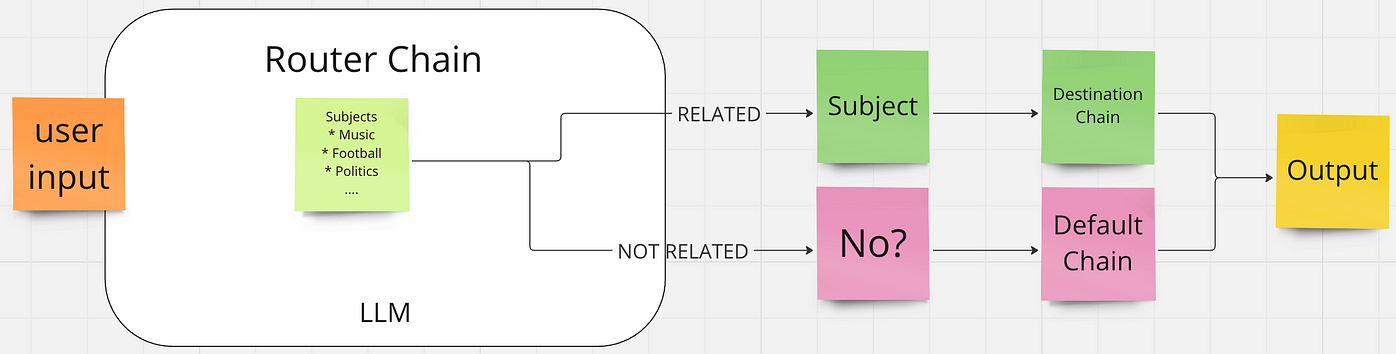
\includegraphics[width=0.8\textwidth]{assets/LangchainRouterChainExample.png}
    \caption{Example of dynamic routing in a chatbot conversation.}
    \label{fig:router_chain_example}
\end{figure}

\section{Existing Solutions and Their Approaches}

\subsection{No-Code Chatbot Builders}
No-code chatbot builders, such as Chatfuel~\cite{chatfuel}, Landbot~\cite{landbot}, and ManyChat~\cite{manychat}, allow users to create structured chatbot flows visually. These tools offer ease of use but are heavily reliant on predefined responses, which limits their adaptability to dynamic user input. For instance, they struggle to handle unexpected or unstructured queries, making them less suitable for complex conversational scenarios. While they excel in creating static, rule-based workflows, they lack the flexibility to adapt to more dynamic interactions. ManyChat, for example, is widely used for social media chatbots but is limited in its ability to handle complex, multi-turn conversations or integrate with advanced AI capabilities.

\subsection{Automation and Workflow Platforms}
Platforms like Zapier~\cite{zapier} and n8n~\cite{n8n} focus on workflow automation by connecting various services based on triggers and actions. While they excel in automating tasks, they do not offer built-in conversational capabilities or manage continuous user interactions. They can integrate with external tools, but they lack native support for multi-turn, context-aware conversations, limiting their use in chatbot development. These platforms are better suited for back-end automation rather than front-end conversational interfaces.

\subsection{NLP-Powered AI Chatbots}
Dialogflow~\cite{dialogflow} and Rasa~\cite{rasa} provide powerful NLP-driven chatbot solutions that utilize natural language processing (NLP) to understand user intent. These tools are highly adaptable and can handle dynamic user input, but often require significant technical expertise to set up and maintain. Furthermore, their reliance on AI and machine learning makes them unsuitable for users seeking simpler rule-based solutions. While they excel in handling unstructured conversations, they may be overkill and too advanced for simpler use cases.

\subsection{Hybrid Models}
Hybrid chatbot frameworks, such as Botpress~\cite{botpress} and Azure Bot Service~\cite{azurebot}, attempt to merge static workflows with dynamic adaptability. However, these solutions often require extensive manual setup and struggle to achieve a seamless balance between rule-based logic and dynamic interactions. For example, Botpress allows for custom scripting and integration with NLP models, but still prioritizes rule-based logic in many cases. Similarly, Azure Bot Service provides tools for integrating advanced capabilities, but the process can be complex and time-consuming, limiting its effectiveness for users who need simpler, more straightforward solutions.

\section{Identified Gaps in Existing Solutions}
The review of existing solutions reveals several key gaps in the current landscape of chatbot development tools:

\begin{itemize}
    \item \textbf{Integration of Static and Dynamic Approaches}: While some tools excel in creating static, rule-based workflows (e.g., Chatfuel, Landbot) and others specialize in dynamic, AI-driven interactions (e.g., Dialogflow, Rasa), there is no unified solution that seamlessly combines the predictability of static chatbots with the adaptability of dynamic, LLM-powered responses. This fragmentation limits the ability to create chatbots that are both structured and flexible.
    
    \item \textbf{Limited Chatbot Customization}: Many platforms offer limited options for customizing the design and user interface of chatbots. For example, while tools like ManyChat allow for basic branding changes, they lack advanced customization features such as tailored layouts, interactive elements, or personalized themes. This restricts users from creating chatbots that align with their brand identity or user experience goals.
    
    \item \textbf{Customization and Extensibility}: Some platforms offer customization features, but they are often limited in scope or require technical expertise. Additionally, while certain tools allow for extensibility through integrations, there is no unified marketplace or ecosystem where users can easily share, discover, and extend chatbot functionalities in a collaborative manner.
    
    \item \textbf{Publishing and Deployment Options}: Many tools provide basic publishing options, such as embedding chatbots on websites, but lack flexible deployment methods like APIs or marketplace listings. This inconsistency limits the accessibility and reusability of chatbots across different platforms and use cases.
    
    \item \textbf{High Complexity in Setup and Maintenance}: Tools that offer advanced features, such as NLP or hybrid models (e.g., Botpress, Azure Bot Service), often require significant technical expertise and manual configuration. While these tools are powerful, their complexity creates a barrier for non-technical users who need simpler, more intuitive solutions.
\end{itemize}

\section{Proposed Approach: FlowX}
FlowX addresses these gaps by offering a unique approach to chatbot development that combines the strengths of static and dynamic workflows while providing additional features for customization, extensibility, and deployment. The key aspects of FlowX's approach include:

\begin{itemize}
    \item \textbf{Seamless Integration of Static and Dynamic Capabilities}: FlowX enables users to create structured, rule-based chatbot flows while integrating dynamic, LLM-powered responses where needed. This hybrid approach allows for predictable, controlled interactions as well as adaptability to unstructured user input, bridging the gap between static and dynamic chatbot development.
    
    \item \textbf{Advanced Chatbot Customization}: FlowX provides extensive customization options for chatbot design, enabling users to tailor the look and feel of their chatbots to match their brand identity or user experience goals. Users can customize layouts, colors, fonts, and interactive elements, ensuring that chatbots are not only functional but also visually appealing and engaging.
    
    \item \textbf{Comprehensive Marketplace and Extensibility Features}: FlowX introduces a marketplace where users can discover, share, and extend chatbot functionalities. This ecosystem promotes collaboration and reusability, allowing users to customize their chatbots with pre-built components or share their own creations with the community. Unlike existing tools, FlowX provides a unified platform for both customization and extensibility.
    
    \item \textbf{Flexible Publishing Options}: FlowX provides multiple options for publishing chatbots, including deployment as APIs and listing on the marketplace. This flexibility ensures that chatbots can be easily integrated into various platforms and made accessible to a wider audience, addressing the limitations of existing tools that offer only basic publishing options.
    
    \item \textbf{User-Friendly Design}: FlowX prioritizes ease of use, enabling both technical and non-technical users to create, customize, and deploy chatbots without requiring extensive setup or maintenance. The platform's intuitive interface and guided workflows reduce the complexity often associated with chatbot development, making it accessible to a broader range of users.
\end{itemize}

By addressing these gaps, FlowX aims to provide a comprehensive solution that bridges the divide between static and dynamic chatbot development while fostering a collaborative ecosystem for innovation and reuse.

\section{Conclusion}
This literature review highlights the strengths and limitations of existing chatbot building tools, automation platforms, and AI-driven frameworks. Although some tools offer partial solutions, none provide a comprehensive approach that integrates structured flow-building with the power of LLM-based responses, alongside features such as advanced customization, a marketplace, robust extensibility, and flexible publishing options. FlowX addresses these challenges by combining the best of both worlds, creating a more flexible, intelligent, and user-friendly chatbot development experience.

\chapter{Methodology}
\section{Chatbot Builder}

\subsection {Initial Design}
The Chatbot Builder is a web application that allows users to create chatbot workflows using a visual interface. This interface consists of a canvas where users can drag and drop nodes to create a flowchart-like structure. Each node represents a step in the chatbot conversation, and connections between nodes represent the flow of the conversation.

The following figure shows our initial design for the Chatbot Builder interface:

\begin{figure}[H]
    \centering
    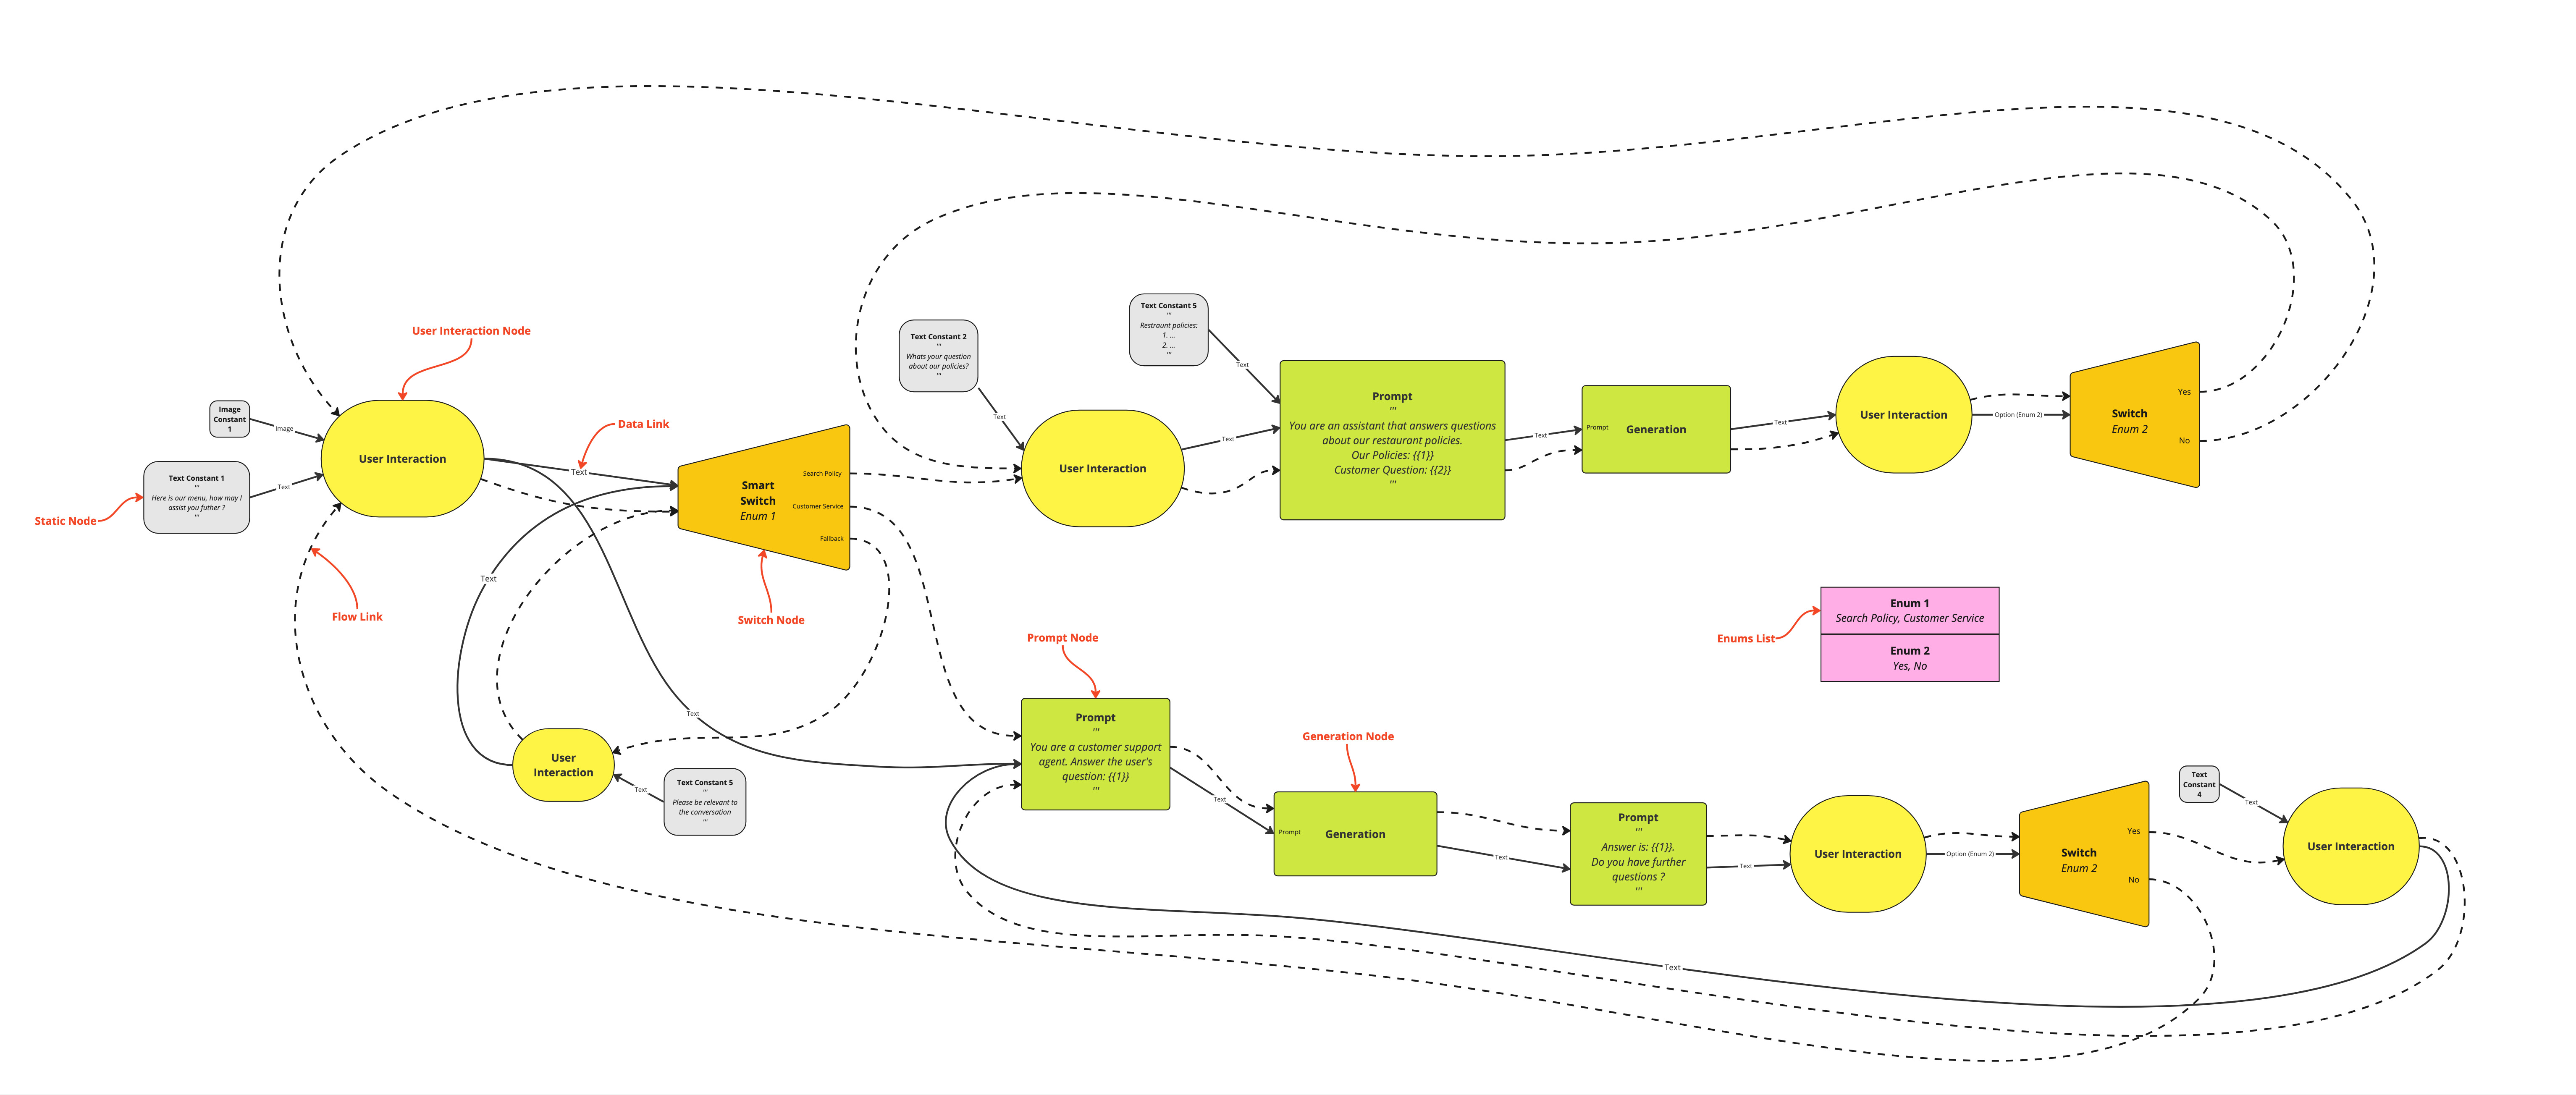
\includegraphics[width=0.95\textwidth]{assets/ChatbotBuilder_Sketch.jpg}
    \caption{Initial design of the Chatbot Builder interface}
    \label{fig:chatbot_builder}
\end{figure}

The design shows the following components:
\begin{itemize}
    \item \textbf{User Interaction Node}: Represents a user input node where the chatbot waits for user input.
    \item \textbf{Switch Node}: Represents a conditional node where the chatbot can branch based on a given option.
    \item \textbf{Prompt Node}: Represents a text template with placeholders for dynamic content at runtime.
    \item \textbf{Generation Node}: Represents a node that generates dynamic content using a language model.
    \item \textbf{Static Node}: Represents a constant value that is passed to other nodes.
    \item \textbf{Smart Switch Node}: Represents a conditional node that can branch based on the output of a language model, AKA Dynamic Routing.
    \item \textbf{Data Link}: Represents a connection between nodes that carries data from one node to another.
    \item \textbf{Flow Link}: Represents a connection between nodes that defines the flow of the conversation.
\end{itemize}


\subsection{Design Decisions}

\begin{itemize}
    \item In this design we had to add two types of links, Data Link and Flow Link, this is because data is not always passed between nodes in a linear fashion, sometimes data is passed between nodes that are not directly connected in the flow of the conversation.
    \item To ensure logical easy to understand design, we choose an Eager-Evaluation approach where the data is passed through data links as soon as the node finishes its execution. Lazy-Evaluation approach is hard to understand and debug, as the data is passed only when needed, which makes it hard to track the data flow.
    \item Also notice that in this design we have exactly one User node (Interaction Node) instead of separate Input and Output nodes, this is because the chatbot follows a request-response model, where the user sends a request and the chatbot responds with a message, so there won't be any case where the user input isn't followed directly.
\end{itemize}

\subsection{Conversation Flow}

\subsubsection{On Creation Request}
\begin{itemize}
    \item All static nodes are visited (In the order of their IDs), and their values are pushed through their output data links.
    \item Static nodes are of no use after that through out the whole conversation.
    \item Then the start (User Interaction) node is activated by returning output to  user in the response, then the server waits for the next request.
\end{itemize}

\subsubsection{On Further Requests}
\begin{itemize}
    \item Flow control resumes from the user interaction node which the server stopped on last time.
    \item User input is pushed through the node's output data links.
    \item Flow control moves to the next node through the node's flow link.
    \item The following nodes consecutively: activate, push their data, and move flow control. Until the server eventually hit another user interaction node.
    \item Output is finally returned to the user in the response. And the server waits for the next request.
\end{itemize} 

\section{System Design and Architecture}

\subsection{Overview of the System}
The following figure shows an overview of the system architecture of FlowX.
Refer to each microservice's section for more details on the implementation.

\begin{figure}[H]
    \centering
    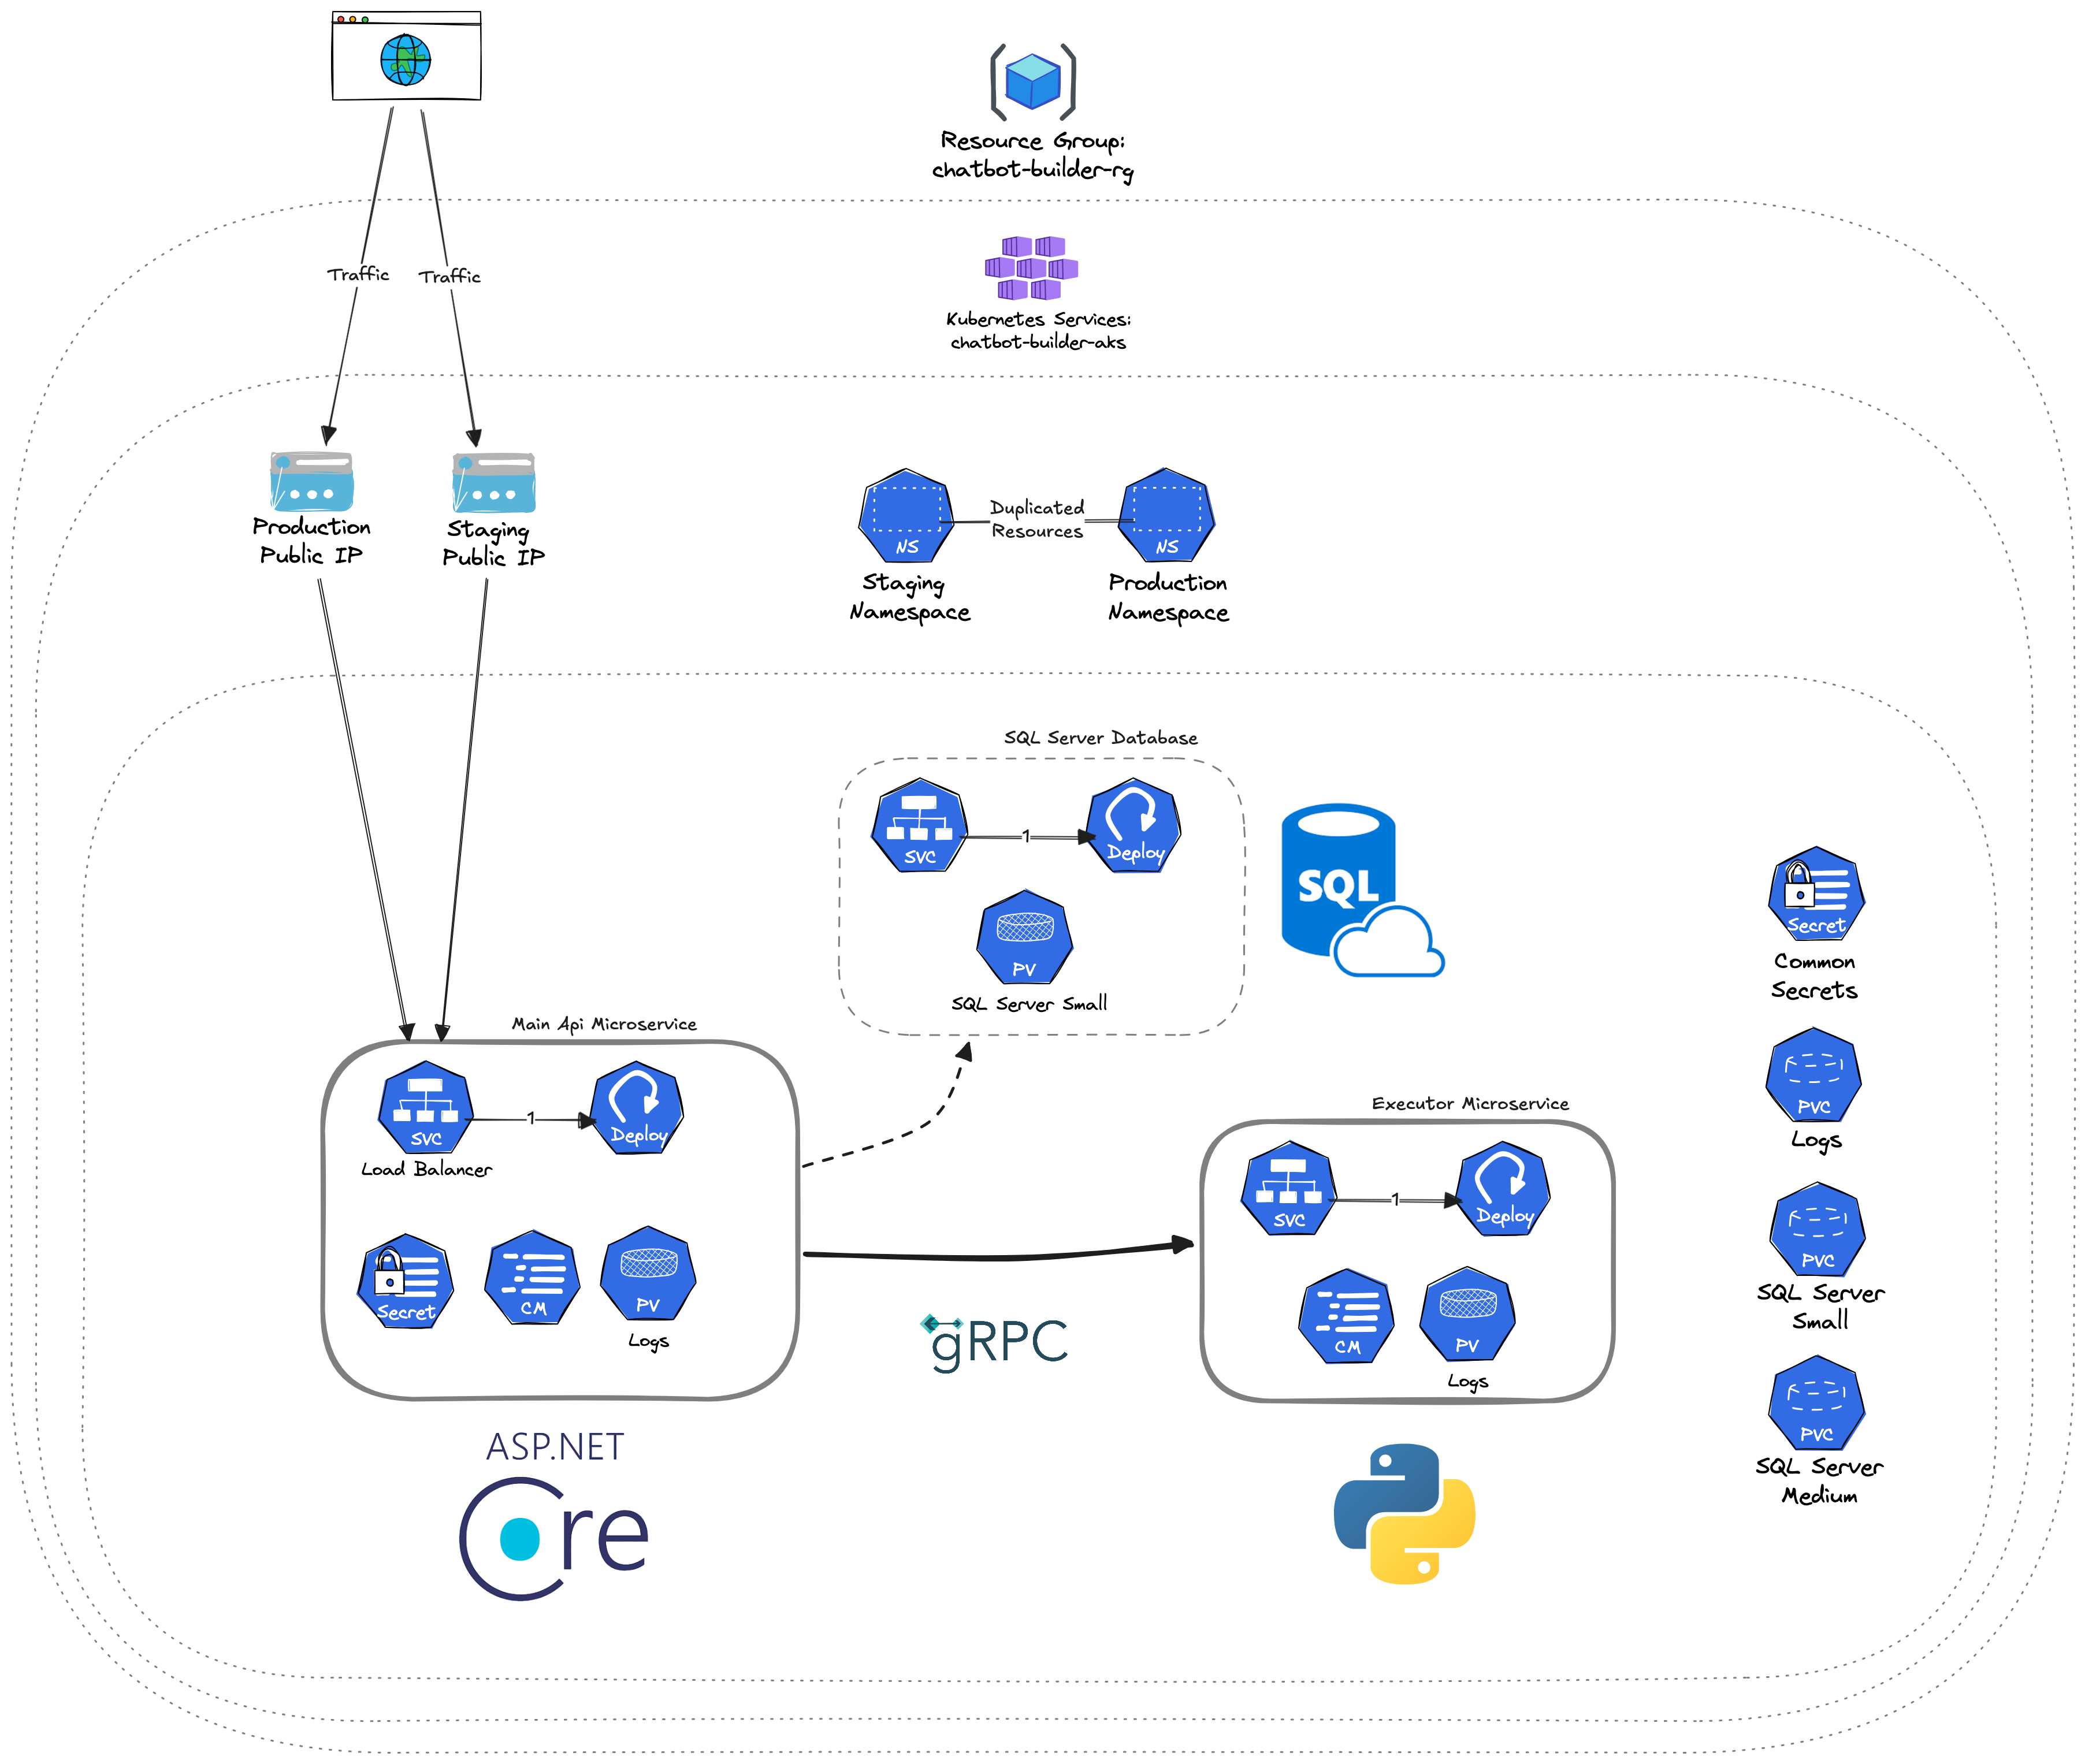
\includegraphics[width=0.95\textwidth]{assets/SystemDesign.png}
    \caption{Microservices architecture of FlowX}
    \label{fig:system_design}
\end{figure}

The project was developed using a microservices architecture, with separate repositories for each microservice and the frontend client. The repositories are as follows:
\begin{itemize}
    \item \textbf{chatbot-builder-api}: The main API microservice for the Chatbot Builder application. Responsible for authentication and orchestrating workflows traversal \& state-management, uses the Executor-Service for LangChain logic.
    \item \textbf{chatbot-builder-executor}: The LangChain execution microservice for the Chatbot Builder application. Controlled by the API-Service, responsible for executing LangChain logic in workflows.
    \item \textbf{chatbot-builder-infra}: Infrastructure \& deployment of the Chatbot Builder application using Terraform \& Kubernetes.
    \item \textbf{chatbot-builder-client}: The frontend for the Chatbot Builder application, built with React Native.
    \item \textbf{chatbot-builder-protos}: Protocol Buffers schema definitions for gRPC communication between API and Executor services.
\end{itemize}

\subsection{API Microservice}
This is the main API microservice for the Chatbot Builder application. It is responsible for authentication and orchestrating workflows traversal \& state-management.

Implemented using ASP.NET Core, which provides a robust strongly typed framework that is easy to maintain and scale.

The following is a few of the key features of the API microservice:
\begin{itemize}
    \item Authentication: JWT-based authentication for user management.
    \item Workflow Management: CRUD operations for workflows, nodes, and connections.
\end{itemize}

\subsection{Executor Microservice}
This is the LangChain execution microservice for the Chatbot Builder application. It is controlled by the API-Service and is responsible for executing LangChain logic in workflows.

Implemented using Python, which contains the Langchain library that abstracts LLM model management and execution.

The following is a few of the key features of the Executor microservice:
\begin{itemize}
    \item gRPC Service: Allows for calls from the API service to execute LangChain logic.
\end{itemize}
\section{Backend}

\subsection{Overview}
The backend of FlowX uses a microservices architecture for scalability and modularity. It consists of:
\begin{itemize}
\item \textbf{API Microservice}: Handles authentication, workflow, and state management.
\item \textbf{Executor Microservice}: Executes LangChain logic.
\item \textbf{Infrastructure Service}: Manages deployment with Terraform and Kubernetes.
\end{itemize}

The following figure shows the API schema for the backend that allows Workflow creation:
\begin{figure}[H]
    \centering
    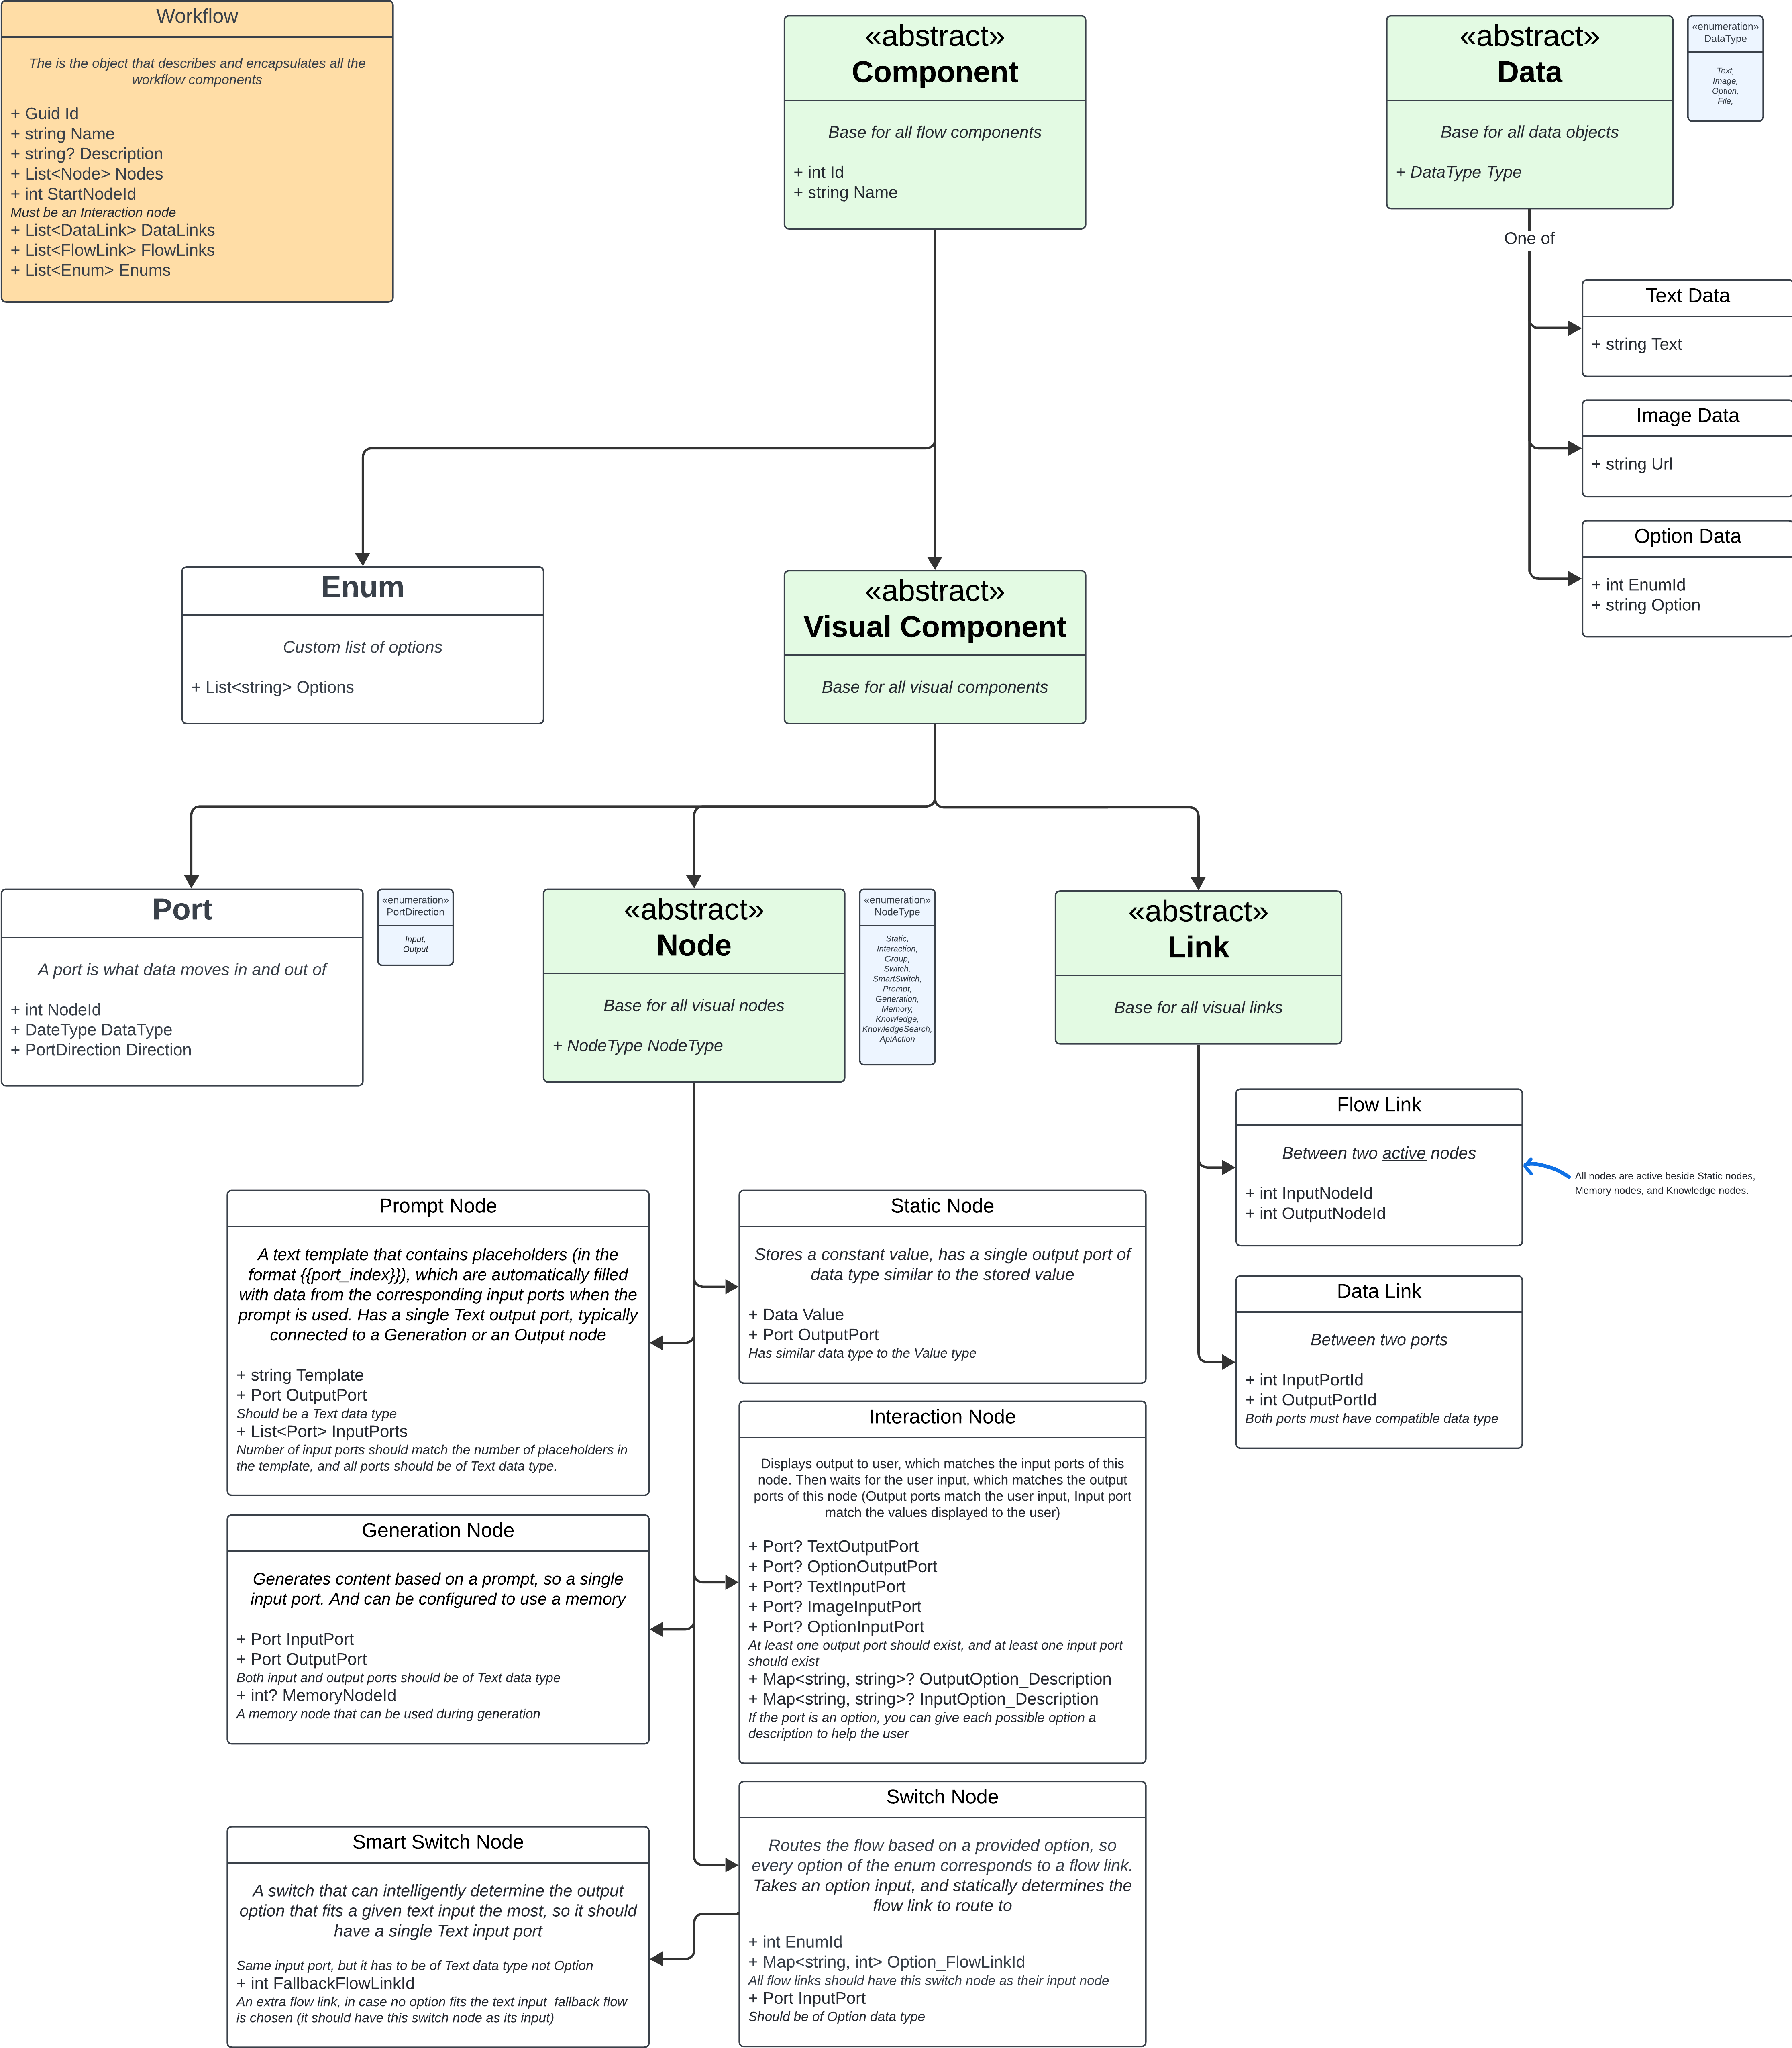
\includegraphics[width=0.95\textwidth]{assets/ChatbotBuilderApiSchema}
    \caption{API Schema for Chatbot Builder Workflows}
    \label{fig:api_schema}
\end{figure}

\subsection{API Microservice}
Built with \textbf{ASP.NET Core}, this service handles:
\begin{itemize}
\item \textbf{Authentication}: Uses JWT-based security.
\item \textbf{Workflow Management}: Supports CRUD operations.
\item \textbf{State Management}: Tracks chatbot workflow states.
\item \textbf{Executor Communication}: Delegates execution via gRPC.
\end{itemize}

\subsection{Domain Model}
The API service implements a rich domain model to support both user management and chatbot workflow functionality. Figure \ref{fig:system_uml} shows the core domain entities and their relationships.

\begin{figure}[H]
    \centering
    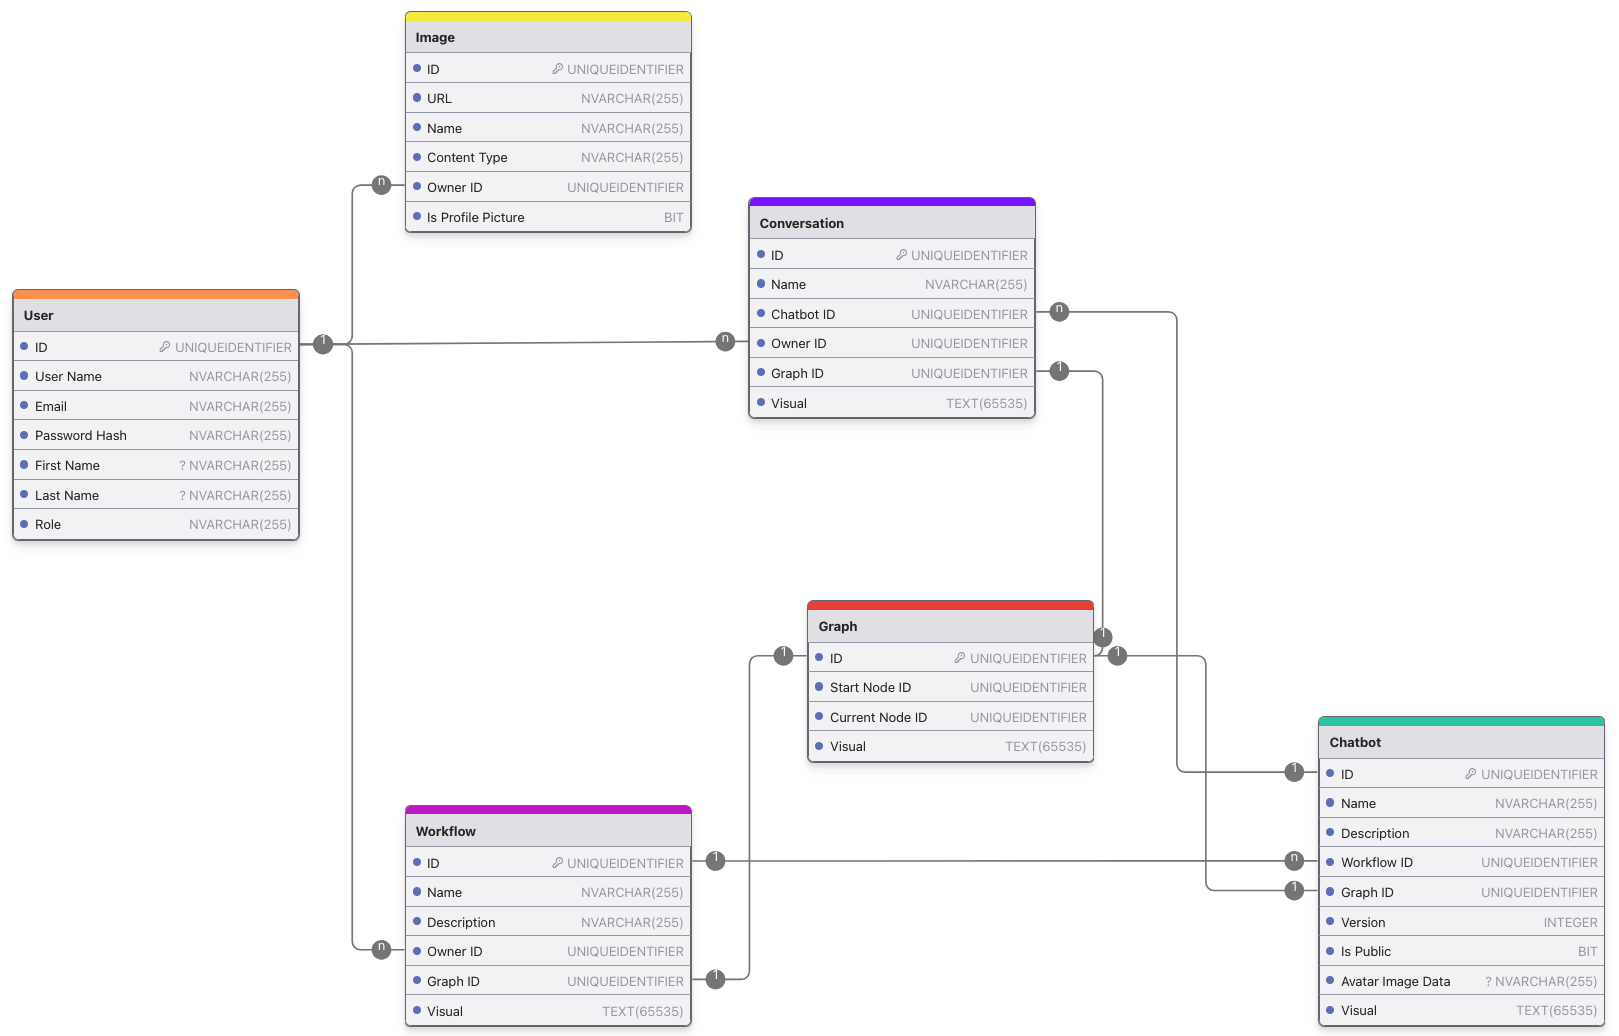
\includegraphics[width=0.95\textwidth]{assets/SystemUmlDiagram.png}
    \caption{Core Domain Model Class Diagram}
    \label{fig:system_uml}
\end{figure}

The domain model is centered around these key entities:
\begin{itemize}
    \item \textbf{User}: Manages authentication and profile data, including role-based access control
    \item \textbf{Chatbot}: Encapsulates chatbot configuration and references to its workflow implementation
    \item \textbf{Workflow}: Contains the complete chatbot logic as a graph structure
    \item \textbf{Graph}: Maintains the topology of nodes and connections that define the chatbot's behavior
    \item \textbf{Conversation}: Handles state management for ongoing user interactions
\end{itemize}

\subsection{Graph Implementation}
The workflow execution engine is built on a sophisticated graph structure (Figure \ref{fig:graph_uml}) that enables both static flows and dynamic LLM-powered interactions.

\begin{figure}[H]
    \centering
    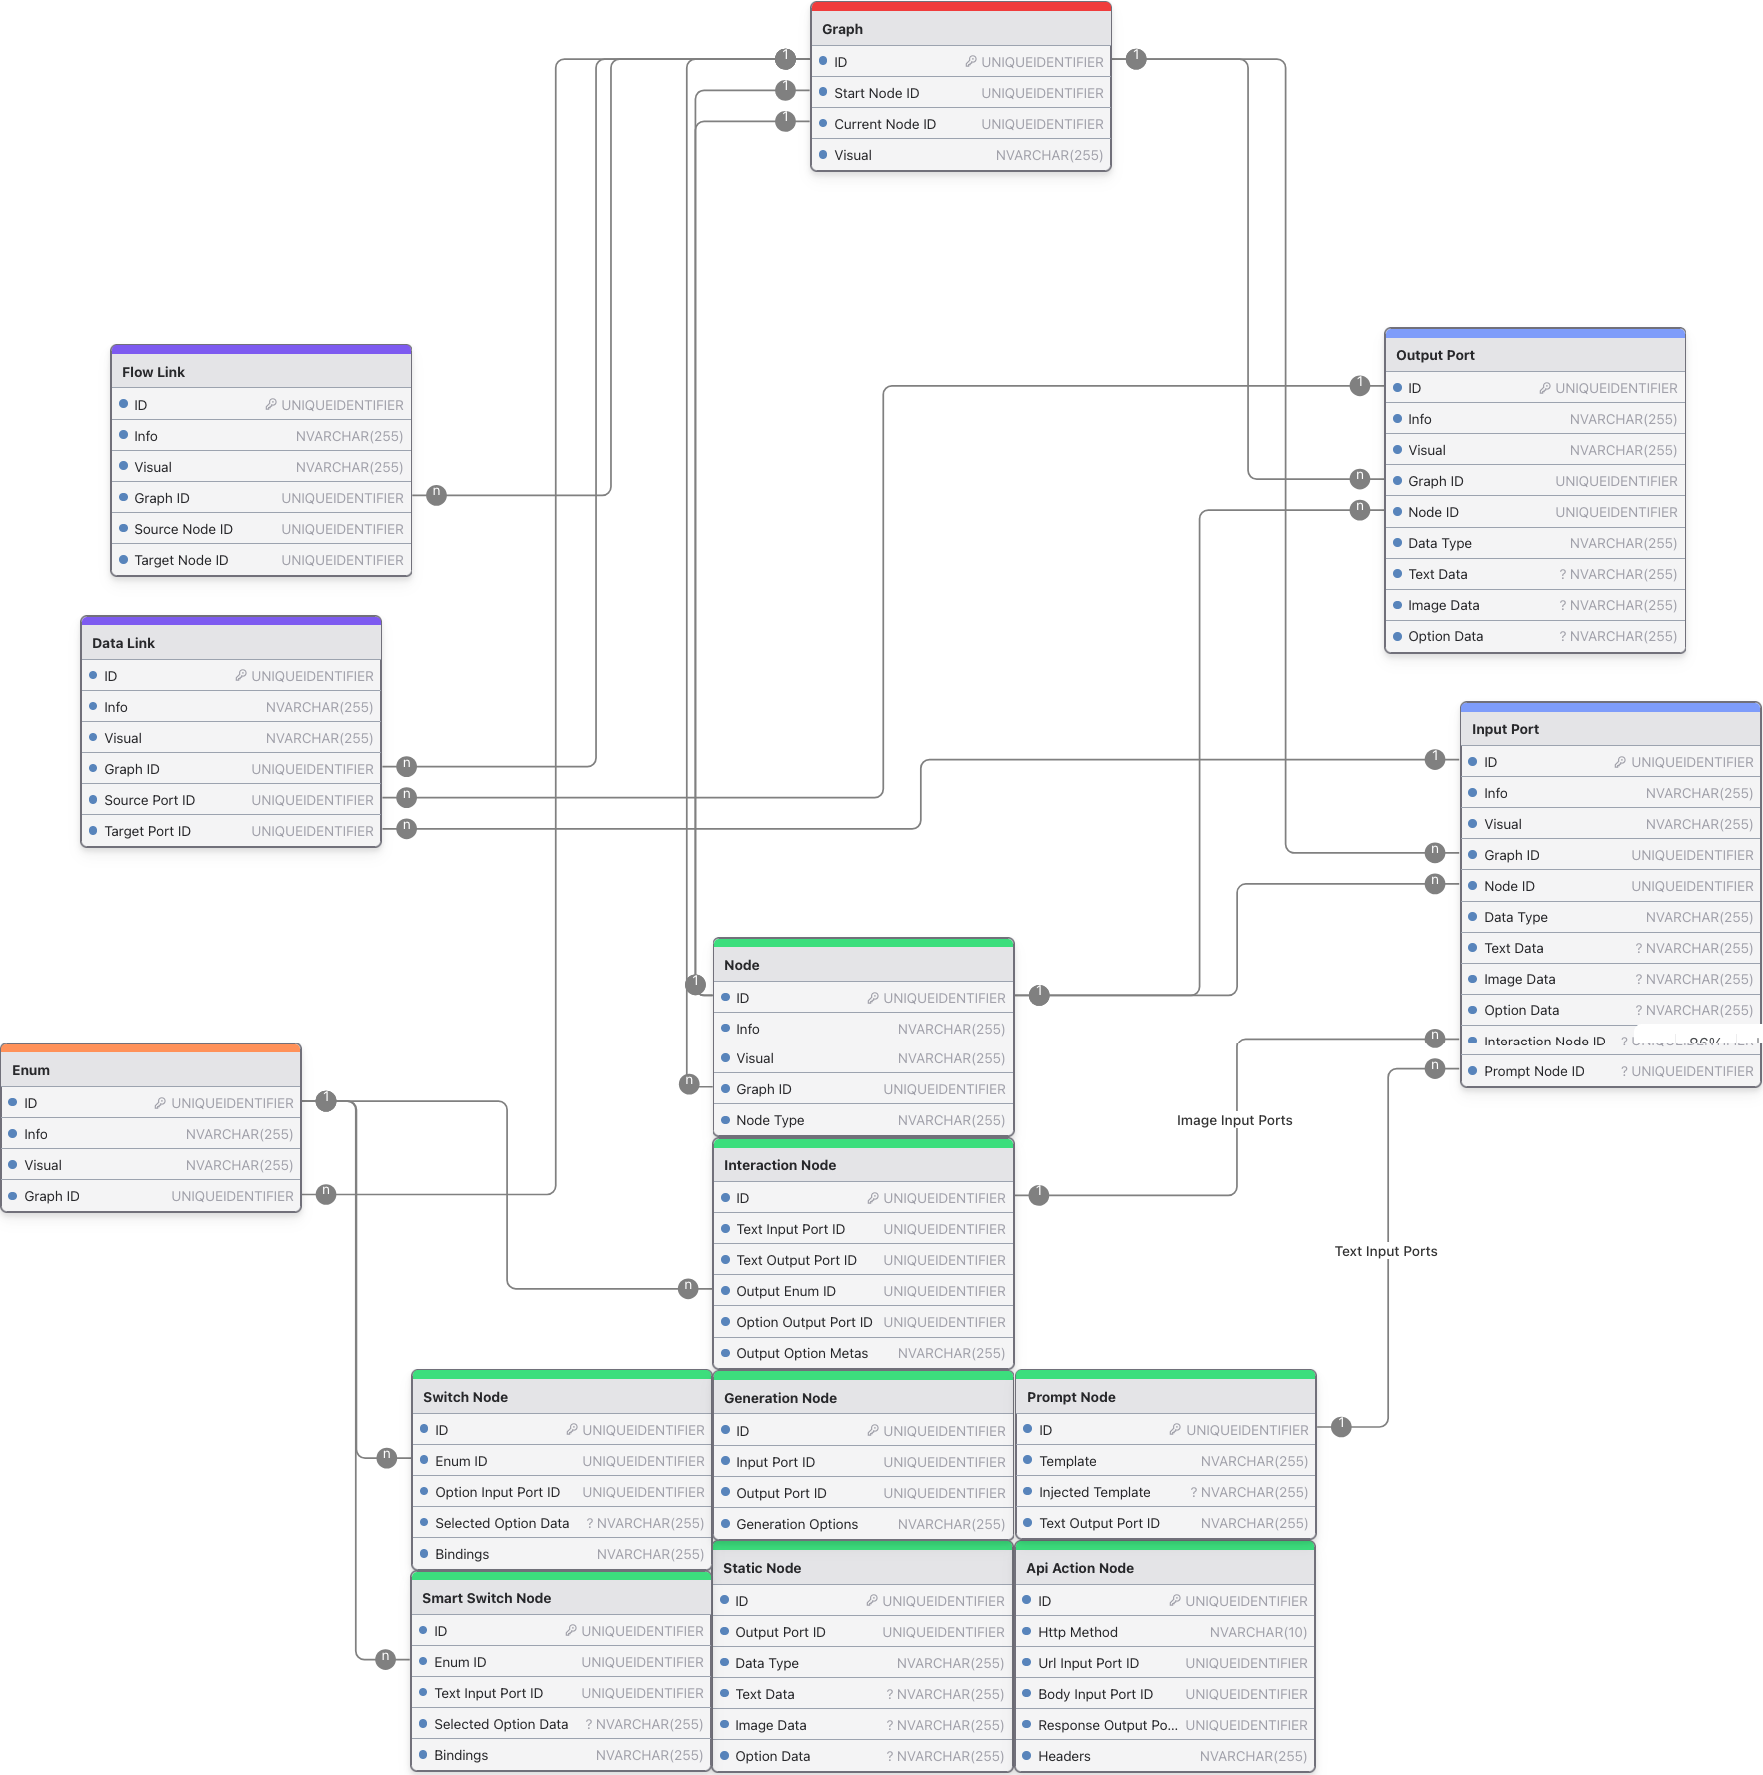
\includegraphics[width=0.95\textwidth]{assets/GraphUmlDiagram.png}
    \caption{Graph Implementation Class Diagram}
    \label{fig:graph_uml}
\end{figure}

The graph implementation includes:
\begin{itemize}
    \item \textbf{Node}: Abstract base class defining common node behavior
    \item \textbf{Input/Output Ports}: Strongly-typed connection points enabling type-safe data flow
    \item \textbf{Flow/Data Links}: Distinct connection types for control flow vs data transfer
    \item \textbf{Specialized Nodes}:
    \begin{itemize}
        \item \textbf{Interaction Node}: Manages user input/output with templating support
        \item \textbf{Generation Node}: Interfaces with the Executor service for LLM operations
        \item \textbf{Switch Node}: Implements both static and LLM-powered conditional branching
        \item \textbf{Static Node}: Provides deterministic responses
        \item \textbf{API Action Node}: Enables integration with external services
    \end{itemize}
\end{itemize}

\subsection{Executor Microservice}
Developed in \textbf{Python} with \textbf{LangChain}, responsible for:
\begin{itemize}
\item \textbf{Chatbot Logic Execution}.
\item \textbf{gRPC Communication} with the API service.
\item \textbf{Handling Smart Switch Nodes} using LLM outputs.
\end{itemize}

\subsection{Infrastructure and Deployment}
Managed using \textbf{Terraform} and \textbf{Kubernetes}, ensuring:
\begin{itemize}
\item \textbf{Scalable Deployment}: Kubernetes handles scaling and failover.
\item \textbf{Infrastructure as Code (IaC)}: Terraform automates provisioning.
\item \textbf{Service Communication}: Uses gRPC and RESTful APIs.
\end{itemize}
\section{Frontend}

\subsection{Overview and Architecture}
The frontend of FlowX is built with \textbf{React Native}, providing a cross-platform mobile development solution. The application follows a component-based architecture with clear separation of concerns:
\begin{itemize}
    \item \textbf{Presentation Layer}: React Native components and screens
    \item \textbf{State Management}: Redux store with middleware for side effects
    \item \textbf{Service Layer}: API client and WebSocket handlers
    \item \textbf{Utils}: Helper functions and shared utilities
\end{itemize}

\subsection{Visual Workflow Builder}
The core of the application is the visual workflow builder, implemented with several specialized components:

\begin{itemize}
    \item \textbf{Canvas Management}:
    \begin{itemize}
        \item Infinite canvas with pan and zoom capabilities
        \item Grid-based snapping for precise node placement
        \item Multi-select and bulk operations
    \end{itemize}
    
    \item \textbf{Node System}:
    \begin{itemize}
        \item Drag-and-drop node creation and positioning
        \item Smart port connection system with type validation
        \item Real-time node state visualization
        \item Custom node templates for different interaction types
        \item Bezier curve connections with interactive editing
    \end{itemize}

    \item \textbf{Node Editor}:
    \begin{itemize}
        \item Rich text editor for message templates
        \item Dynamic form generation for node configuration
        \item Each node with its own properties
    \end{itemize}
    
    \item \textbf{Chat Designer}:
    \begin{itemize}
        \item Live preview of chatbot behavior
        \item Mobile-first chat interface
        \item Allows for designing the visuals of the chatbot
    \end{itemize}
\end{itemize}

\subsection{State Management and Performance}
The application uses Redux for state management with several optimizations for performance:

\begin{itemize}
    \item \textbf{Store and Updates}:
    \begin{itemize}
        \item Normalized state shape for efficient updates
        \item Separate slices for UI state and domain data
        \item Optimistic updates for better responsiveness
        \item Redux Thunk for async operations
        \item Persistence middleware for auto-saving
    \end{itemize}
    
    \item \textbf{Performance Optimizations}:
    \begin{itemize}
        \item Virtual scrolling for large workflows
        \item Lazy loading of node components
        \item Memoization of expensive computations
        \item Batched updates for multiple changes
        \item Debounced save operations
        \item Selective re-rendering using React.memo
    \end{itemize}
\end{itemize}

\subsection{Cross-Platform Design}
The application ensures consistent behavior across platforms through:

\begin{itemize}
    \item \textbf{Responsive Design}:
    \begin{itemize}
        \item Platform-specific UI adjustments
        \item Adaptive layouts for different screen sizes
    \end{itemize}
\end{itemize}
\section{Infrastructure}
\label{sec:infrastructure}

\subsection{Architectural Approach}
The infrastructure was designed using Infrastructure-as-Code (IaC) principles with three core components:

\begin{itemize}
    \item \textbf{Terraform}: For provisioning cloud resources on Azure, leveraging Terraform Cloud for state management.
    \item \textbf{Kubernetes}: For container orchestration and deployment management using Azure Kubernetes Service (AKS).
    \item \textbf{GitHub Actions}: For CI/CD pipeline automation, managing infrastructure provisioning and application deployment.
\end{itemize}

This combination enables reproducible environments and automated deployment processes across staging and production environments.

\subsection{Terraform Implementation}
The Terraform configuration manages the complete Azure infrastructure through modular components:

\begin{itemize}
    \item \textbf{Resource Groups}: Logical containers for Azure resources.
    \item \textbf{AKS Clusters}: Kubernetes clusters with auto-scaling node pools.
    \item \textbf{Blob Storage}: Azure Blob Storage for persistent data storage.
    \item \textbf{Public IPs}: Dedicated IP addresses per environment, injected into Kubernetes manifests.
\end{itemize}

\begin{lstlisting}[language=HCL,caption=Sample Terraform module for AKS]
module "aks" {
  source              = "./modules/aks"
  environment         = "staging"
  node_count         = 3
  vm_size            = "Standard_D2_v2"
  dns_prefix         = "chatbot-builder-staging"
  resource_group_name = azurerm_resource_group.main.name
}
\end{lstlisting}

Terraform outputs include:
\begin{itemize}
    \item \textbf{Kubernetes Configuration}: Kubeconfig file for cluster authentication.
    \item \textbf{Public IPs}: Used for Load Balancers and injected into Kubernetes manifests.
\end{itemize}

\subsection{Kubernetes Orchestration}
The Kubernetes implementation follows a multi-environment strategy using Kustomize:

\begin{itemize}
    \item \textbf{Base Configuration}: Common resources (Pods, Services, Ingress).
    \item \textbf{Environment Overlays}: Staging and Production-specific customizations.
    \item \textbf{Secret Management}: Kubernetes secrets encrypted with SealedSecrets.
\end{itemize}

Deployment follows this phased approach:
\begin{enumerate}
    \item Persistent Volume Claims for storage.
    \item ConfigMaps for environment variables.
    \item Microservice deployments.
    \item Network policies and ingress rules.
\end{enumerate}

Directory structure:
\begin{itemize}
    \item \textbf{base/}: Core manifests including ConfigMaps, PVCs, Deployments, and Services.
    \item \textbf{overlays/}: Staging and production configurations.
    \item \textbf{secrets/}: Templates for Kubernetes secrets, applied manually before automation.
\end{itemize}

\subsection{CI/CD Pipeline}
The CI/CD pipeline is managed with GitHub Actions and follows GitOps principles.
Key workflows:

\begin{itemize}
    \item \textbf{Terraform Deployment}: Runs on changes to the `infra/` directory.
    \begin{itemize}
        \item Initializes Terraform and validates configuration.
        \item Applies infrastructure changes if on `main` branch.
        \item Outputs kubeconfig and public IPs.
    \end{itemize}
    \item \textbf{Kubernetes Deployment}: Triggered via repository dispatch for staging/production.
    \begin{itemize}
        \item Fetches Terraform outputs (Kubernetes config, public IPs).
        \item Updates Kubernetes manifests with correct environment values.
        \item Deploys microservices and infrastructure resources to AKS.
    \end{itemize}
\end{itemize}

\section{Project Management}
The project was managed using Jira~\cite{jira}, a widely adopted Agile project management tool. The development process followed an iterative approach, with tasks organized into epics that represent the major functional areas. Key epics included Technical Setup, Prototype Development, Feature Implementation, and Documentation.

The project was divided into several epics, each representing a major functional area or phase of development. Below is a detailed breakdown of the epics and their associated tasks:

\subsubsection{Epic 1: Technical Aspects}
This epic focused on setting up the foundational technical infrastructure for the project.
\begin{itemize}
    \item CB-4: Setup CI/CD with AKS
    \item CB-6: Setup API-Service Project
    \item CB-5: Setup Executor-Service Project
    \item CB-18: Setup Engine-Service Project
    \item CB-20: Add SqlServer Database to API Service
    \item CB-21: Setup Terraform Project
    \item CB-17: Maintain Kubernetes Manifests
    \item CB-22: Maintain CI/CD Pipeline
    \item CB-23: Maintain Terraform Infrastructure
    \item CB-38: Add MongoDB to Executor Service
\end{itemize}

\subsubsection{Epic 2: Prototype Development}
This epic involved creating the initial prototype and implementing core functionalities.
\begin{itemize}
    \item CB-8: Creating the First Prototype
    \item CB-9: Setup Jwt Authentication in the Api-Service
    \item CB-10: Develop Api Schema
    \item CB-11: Develop gRPC Schema between Api-Service \& Engine-Service
    \item CB-19: Implement Engine-Service Domain
    \item CB-24: Implement Engine-Service Application
    \item CB-13: Implement Api-Service Logic
    \item CB-25: Merge Engine into API Temporarily
\end{itemize}

\subsubsection{Epic 3: Adding Core Features}
This epic focused on adding essential features to the platform.
\begin{itemize}
    \item CB-26: Adding Essential Features
    \item CB-27: Implement User Images Endpoints
    \item CB-29: Add More User Fields
    \item CB-28: Maintain Api Endpoints
    \item CB-30: Add ApiAction Node
    \item CB-12: Develop gRPC Schema between Engine-Service \& Executor-Service
    \item CB-32: Add Generation \& SmartSwitch Nodes
    \item CB-14: Implement Executor-Service Logic
    \item CB-33: Add Image Ports for Interaction Node
\end{itemize}

\subsubsection{Epic 4: Adding Advanced Features}
This epic involved implementing additional advanced features to enhance the platform's capabilities.
\begin{itemize}
    \item CB-35: Adding Extra Features
    \item CB-37: Add ImageData to InteractionOptionMetas
    \item CB-36: Add Avatar Picture to Chatbots
    \item CB-41: Return ProfilePicture with User details
    \item CB-42: Add Object Visual fields
    \item CB-43: Add Chatbot-Graph Query for Owners
    \item CB-31: Add Entities Statistics
\end{itemize}

\subsubsection{Epic 5: Domain Aspects}
This epic focused on project documentation, reporting, and final deliverables.
\begin{itemize}
    \item CB-7: Maintain Pages \& ReadMes
    \item CB-15: Add Workflow Examples
    \item CB-16: Write Project Report
    \item CB-39: Create Demo \& Presentation
\end{itemize}


% \appendix

\bibliographystyle{IEEEtran}
\renewcommand{\bibname}{References}

\bibliography{references}


\end{document}